\begin{center}
\Huge
Logistisk vækst og grafer
\end{center}


\section*{Logistisk vækst og grafer}
\stepcounter{section}

Den eksponentielle differentialligning givet ved
\begin{align*}
	y' = b-ay
\end{align*}
har den grafiske repræsentation set på Fig. \ref{fig:eksp}.
\begin{figure}[H]
	\centering
	\begin{tikzpicture}
		\begin{axis}
			[
			axis lines = center,
			xmin = -1, xmax = 7, 
			ymin = -1, ymax = 7, 
			ticks = none, 
			xlabel = {$y$}, ylabel = {$y'$},
			]
			\addplot[thick, color = blue!50, domain = 0:6] {3-0.5*x};
			\node at (axis cs: 0-0.3,3) {$b$};
			\draw[dashed, color = purple, thick] (axis cs:1,2.5) to (axis cs: 3,2.5);
			\draw[dashed, color = purple, thick] (axis cs:3,2.5) to (axis cs: 3, 1.5);
			\node at (axis cs: 3.3,2) {$a$};
		\end{axis}
	\end{tikzpicture}
	\caption{Grafisk repræsentation af differentialligningen $y' = b-ay$.}
	\label{fig:eksp}
\end{figure}

Vi kan tilsvarende lave en grafisk repræsentation af den logistiske differentialligning
\begin{align*}
	y' = ay(M-y) = -ay^2+aMy.
\end{align*}
Det er ikke svært at overbevise sig om, at dette bliver en "sur" parabel, der skærer i (0,0). Den grafiske repræsentation af denne differentialligning kan ses på Fig. \ref{fig:logist}
\begin{figure}[H]
	\centering
	\begin{tikzpicture}
		\begin{axis}
			[
			axis lines = center, 
			xmin = -1, xmax = 6,
			ymin = -1, ymax = 8,
			ticks = none, 			
			xlabel = {$y$}, ylabel = {$y'$},
			]
			\addplot[color = blue!50, thick, domain = 0:5, samples = 1000] {x*(5-x)};
			\draw[dashed, color = purple, thick] (axis cs: 2.5,0) to (axis cs: 2.5,25/4);
			\node at (axis cs: 2.5, -0.5) {$\frac{M}{2}$};
		\end{axis}
	\end{tikzpicture}
	\caption{Grafisk repræsentation af den logistiske differentialligning $y' = ay(M-y)$.}
	\label{fig:logist}
\end{figure}
Af Fig. \ref{fig:logist} kan vi se, at differentialligningens vækst $y'$ er maksimeret, når $y = M/2$. Dette vil vi vise.
\begin{setn}
	Den logistiske differentialligning 
	\begin{align*}
		y' = ay(M-y)
	\end{align*}
	har maksimal vækst, når $y = M/2$. 
\end{setn}
\begin{proof}
	For at finde toppunktet, differentierer vi polynomiet 
	\begin{align*}
		p(y) =ay(M-y) = aMy-ay^2.
	\end{align*}
	Dette giver
	\begin{align*}
		p'(y) = aM-2ay
	\end{align*}
	Vi sætter dette lig 0 for at finde toppunktet.
	\begin{align*}
		aM-2ay = 0 \ &\Leftrightarrow \ aM = 2ay \\
		&\Leftrightarrow	 \ \frac{aM}{2a} = y \\
		&\Leftrightarrow	 \ \frac{M}{2} = y.
	\end{align*}
\end{proof}

\begin{exa}
	Vi betragter den logistiske differentialligning repræsenteret på Fig. \ref{fig:logist2}.
	\begin{figure}[H]
		\centering
		\begin{tikzpicture}
			\begin{axis}
				[
				axis lines = center, 
				xmin = -1, xmax = 5,
				ymin = -1, ymax = 3, 
				]
				\addplot[thick, color = blue!50, domain = 0:4, samples = 1000] {0.5*x*(4-x)};
				\draw[color = purple, thick, dashed] (axis cs:0,2) to (axis cs: 2,2);
				\draw[color = purple, thick, dashed] (axis cs:2,0) to (axis cs: 2,2);
			\end{axis}
		\end{tikzpicture}
		\caption{Grafisk repræsentation af en logistisk differentialligning.}
		\label{fig:logist2}
	\end{figure}
	Vi kan se, at denne parabel har rødder i 0 og 4. Derfor er differentialligningen på formen
	\begin{align*}
		y' = ay(4-y),
	\end{align*}
	og $M =4$. Vi bestemmer nu toppunktet af parablen.
	\begin{align*}
		a\frac{M}{2}(4-\frac{M}{2}) = a\frac{4}{2}(4-\frac{4}{2}) = a\cdot 2\cdot 2. = 4a
	\end{align*}
	Vi kan af Fig. \ref{fig:logist2} se, at den maksimale vækst er $y' = 2$, så vi må have, at $4a = 2$, og $a=0.5$.
	Vores differentialligning lyder da
	\begin{align*}
		y' = 0.5y(4-y).
	\end{align*}
	Denne differentialligning har den fuldstændige løsning
	\begin{align*}
		y(x) = \frac{4}{1+ce^{-2x}}.
	\end{align*}
\end{exa}

\newpage
\section*{Opgave 1}
Bestem fuldstændige løsninger til følgende grafisk repræsenterede differentialligninger.
\begin{center}
	\resizebox{0.45\textwidth}{!}
	{
		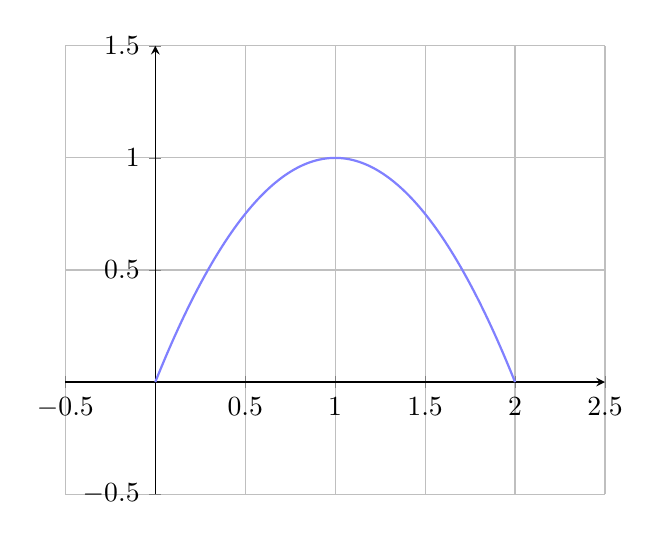
\begin{tikzpicture}
			\begin{axis}
				[
				axis lines = center, 
				xmin = -0.5, xmax = 2.5,
				ymin = -0.5, ymax = 1.5, 
				grid
				]
				\addplot[thick, color = blue!50, domain = 0:2, samples = 1000] {x*(2-x)};
			\end{axis}
		\end{tikzpicture}
	}
	\resizebox{0.45\textwidth}{!}
	{
		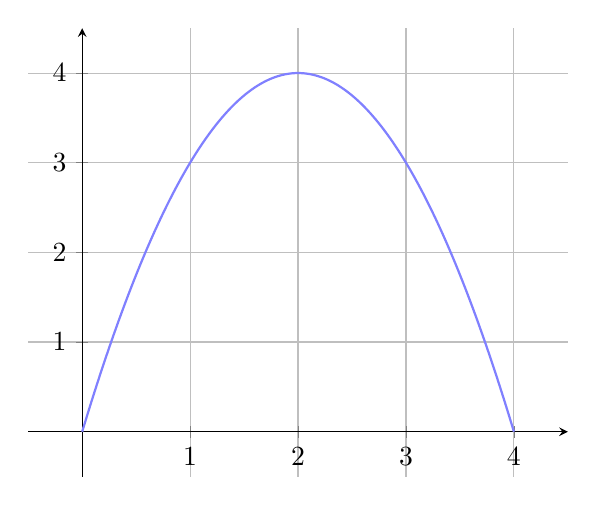
\begin{tikzpicture}
			\begin{axis}
				[
				axis lines = center, 
				xmin = -0.5, xmax = 4.5,
				ymin = -0.5, ymax = 4.5, 
				grid
				]
				\addplot[thick, color = blue!50, domain = 0:4, samples = 1000] {x*(4-x)};
			\end{axis}
		\end{tikzpicture}
	}
	\resizebox{0.45\textwidth}{!}
	{
		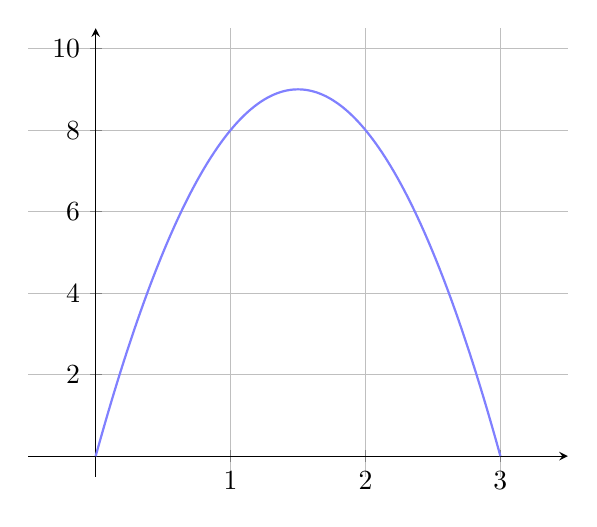
\begin{tikzpicture}
			\begin{axis}
				[
				axis lines = center, 
				xmin = -0.5, xmax = 3.5,
				ymin = -0.5, ymax = 10.5, 
				grid
				]
				\addplot[thick, color = blue!50, domain = 0:3, samples = 1000] {4*x*(3-x)};
			\end{axis}
		\end{tikzpicture}
	}	
	\resizebox{0.45\textwidth}{!}
	{
		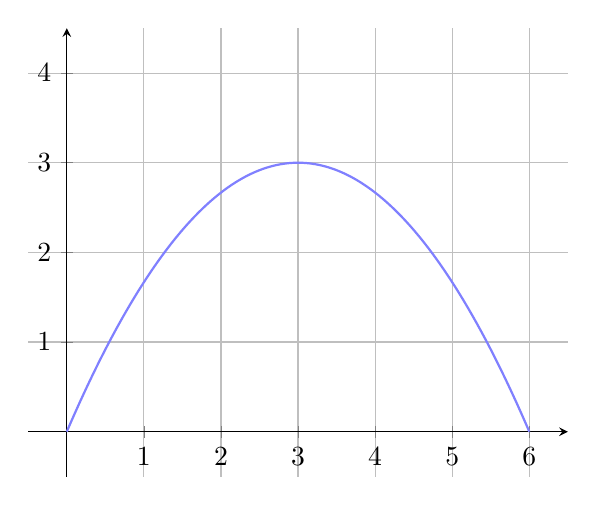
\begin{tikzpicture}
			\begin{axis}
				[
				axis lines = center, 
				xmin = -0.5, xmax = 6.5,
				ymin = -0.5, ymax = 4.5, 
				grid
				]
				\addplot[thick, color = blue!50, domain = 0:6, samples = 1000] {(1/3)*x*(6-x)};
			\end{axis}
		\end{tikzpicture}
	}	
\end{center}
\newpage
\section*{Opgave 2}
\begin{enumerate}[label=\roman*)]
	\item Bestem en fuldstændig løsning til følgende grafisk repræsenterede differentialligning.
	\begin{center}
		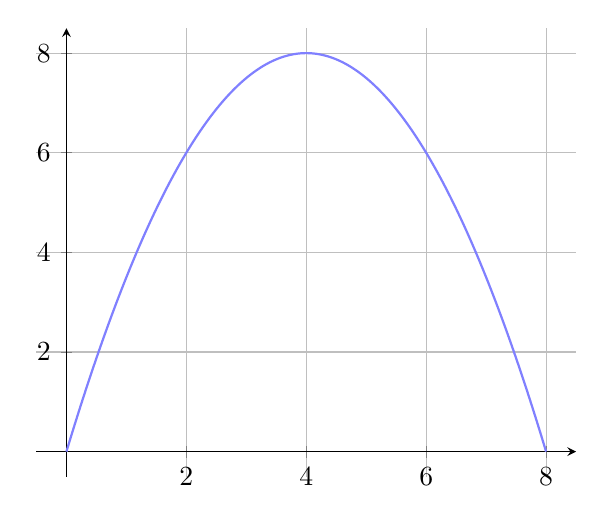
\begin{tikzpicture}
			\begin{axis}
				[
				axis lines = center, 
				xmin = -0.5, xmax = 8.5,
				ymin = -0.5, ymax = 8.5, 
				grid
				]
				\addplot[thick, color = blue!50, domain = 0:8, samples = 1000] {0.5*x*(8-x)};
			\end{axis}
		\end{tikzpicture}
	\end{center}
	\item Bestem nu en partikulær løsning, der går gennem punktet $(0,4)$. 
	\item Hvad er væksten af $y$, når $y=5$?
	\item Bestem $y(2)$. 
\end{enumerate}
\newpage
\section*{Opgave 3}
\begin{enumerate}[label=\roman*)]
	\item Bestem en fuldstændig løsning til følgende grafisk repræsenterede differentialligning.
	\begin{center}
		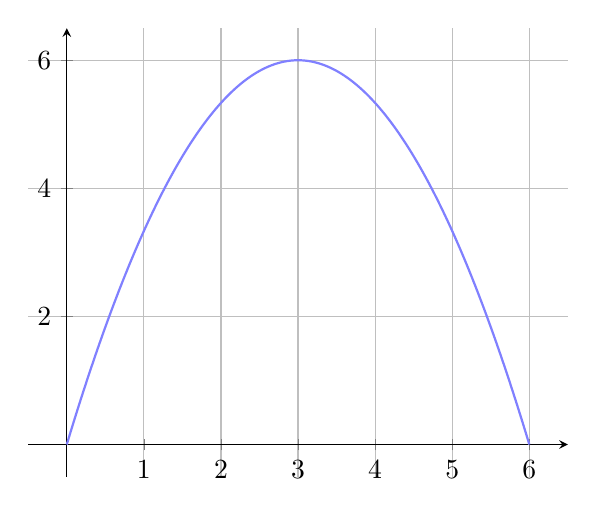
\begin{tikzpicture}
			\begin{axis}
				[
				axis lines = center, 
				xmin = -0.5, xmax =6.5 ,
				ymin = -0.5, ymax = 6.5, 
				grid
				]
				\addplot[thick, color = blue!50, domain = 0:6, samples = 1000] {(2/3)*x*(6-x)};
			\end{axis}
		\end{tikzpicture}
	\end{center}
	\item Bestem nu en partikulær løsning, der går gennem punktet $(0,12)$.
	\item Hvad er væksten af $y$, når $y=2$?
	\item Bestem $y(4)$.  
\end{enumerate}
